% Chapter Template

\chapter{Modelo con LSTM} % Main chapter title

\label{LSTM} % Change X to a consecutive number; for referencing this chapter elsewhere, use \ref{ChapterX}

%----------------------------------------------------------------------------------------
%   SECTION 1
%----------------------------------------------------------------------------------------

\section{Herramientas}

Para desarrollar la implementaci\'on con LSTM se utiliz\'o el framework en python llamado Keras, que
implementa abstracciones sencillas para crear modelos de redes con distintas capas, utilizando
Tensorflow o Theano.

Si bien permite realizar desarrollos y pruebas de forma r\'apida, no tiene el nivel de ajuste tan
bajo nivel como utilizar directamente Theano o Tensorflow.

Todos los modelos fueron entrenados monitoreando el MSE (y la precisi\'on en los modelos por
clasificaci\'on), al mismo tiempo que se verificaba el ``desempe\~no'' en el set de cross-validation
para controlar el overfitting.

\begin{figure}[h]
    \centering
    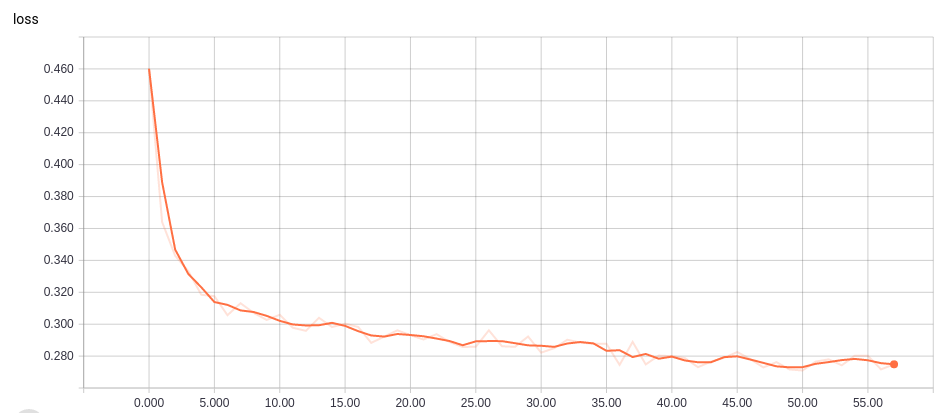
\includegraphics[width=1\linewidth]{Figures/train_loss.png}
    \decoRule
    \caption[Train loss]{El valor del costo en el entrenamiento.}
    \label{fig:Costo durante el entrenamiento}
\end{figure}

\begin{figure}[h]
    \centering
    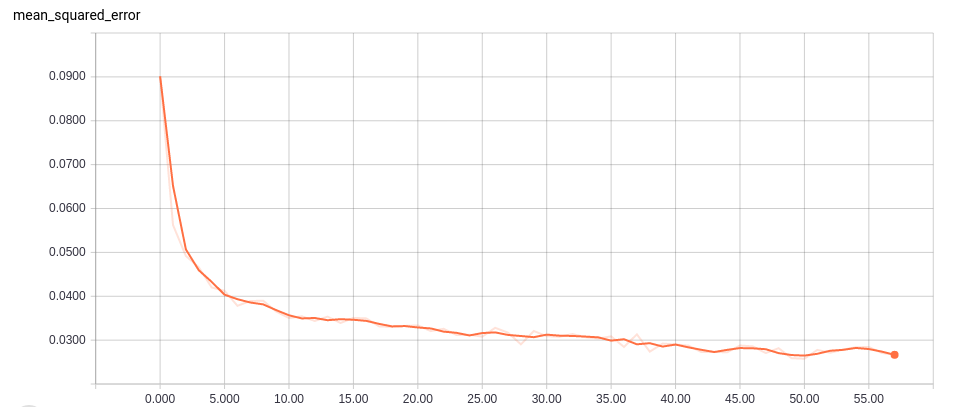
\includegraphics[width=1\linewidth]{Figures/train_mse.png}
    \decoRule
    \caption[MSE]{El valor del MSE en el set de entrenamiento.}
    \label{fig:MSE en el set de entrenamiento}
\end{figure}

\begin{figure}[h]
    \centering
    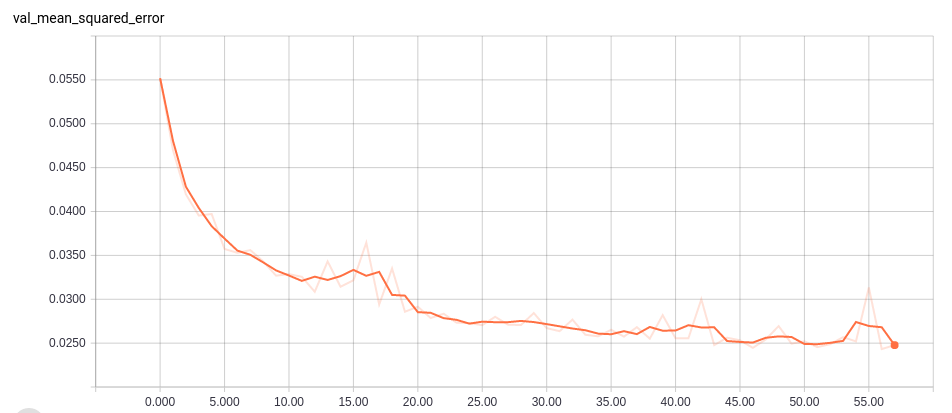
\includegraphics[width=1\linewidth]{Figures/val_mse.png}
    \decoRule
    \caption[Validation MSE]{El valor del MSE en el set de CV luego de cada iteraci\'on.}
    \label{fig:MSE en el set CV}
\end{figure}

%-----------------------------------
%   SUBSECTION 1
%-----------------------------------
\subsection{Limpieza del texto}

Como la cantidad de t\'erminos era enorme (alrededor de 100.000), realizamos un checkeo manual sobre
los textos, viendo que hab\'ia varias URLs, HTML, fechas, horas, comillas, etc. Esto resultaba en
una gran cantidad de tokens que realmente no aportaban demasiado, pero incrementaban el tama\~no de
los vectores encodeados, y por lo tanto  se decidi\'o hacer una limpieza del texto.

Las URLs fueron removidas, asi como tambi\'en el HTML y los separadores como ``---------''.
Las fechas y horas fueron reemplazadas por las palabras ``date'' y ``time'' respectivamente, as\'i
como los n\'umeros por la palabra ``number''. Las repeticiones del signo ``\$'' o los montos
``\$nnn'' fueron reemplazados por la palabra ``money''.

Tambi\'en se removieron las comillas alrededor de las citas, para evitar tokens del tipo `` 'this ''.

Otras pruebas r\'apidas llevaron a concluir que el texto en el campo `Summary' algunas veces
resultaba \'util, por lo que se decidi\'o incluirlo tambi\'en como parte del texto. Se experiment\'o
utilizando configuraciones de redes y entrenandolas con los sets que incluian o ignoraban los
summaries. Por lo general el resultado era mejor cuando se los incly\'o.

%-----------------------------------
%   SECTION 2
%-----------------------------------

\section{LSTM con 1-hot encoding}

Las redes LSTM mantienen un estado interno (``memoria'') lo que permite, a diferencia de las otras,
que la salida dependa no solo de la entrada, sino tambi\'en de las entradas anteriores
\cite{understanding_LSTM}. La forma de entrenarlas que utilizamos fue de a una palabra (encodeada
en un vector) a la vez.
Luego de analizar un review, el estado interno es reseteado. \cite{LSTM_time_series_predictions},
\cite{stateful_LSTM}

En todos los casos, se utiliz\'o entrenemiento por mini-batches para acelerar el proceso. Debido a
esto, hubo que seleccionar un valor fijo de t\'erminos por review.

\begin{figure}[h]
    \centering
    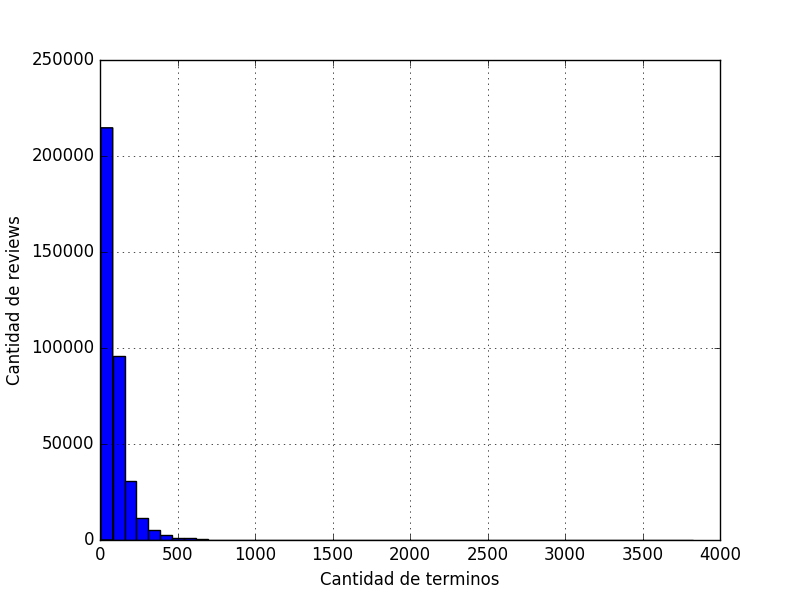
\includegraphics[width=1\linewidth]{Figures/terminos_por_review.png}
    \decoRule
    \caption[Terminos por review]{Histograma del largo de los reviews (por t\'erminos).}
    \label{fig:Histograma del largo de los reviews (por t\'erminos)}
\end{figure}

Debido a la cantidad de memoria requerida, no se pudo utilizar el largo mas grande (3826), por lo
que decidimos elegir 400, que abarcaba la gran mayoria. Los reviews de mayor longitud fueron
truncados, y los mas cortos paddeados con ceros al principio.

La primera prueba fue un modelo b\'asico que consis\'ia simplemente en 1 capa de 60 neuronas LSTM,
recibiendo las palabras en un 1-hot encoding, ignorando stop words. Este modelo ten\'ia 1 neurona
con funci\'on de activaci\'on sigmoidal como salida para obtener un resultado en el rango 0-1.

El modelo logr\'o un buen resultado para su simpleza (alrededor de 0.7 MSE en pruebas locales con el
set de cross-validation).

Agregando una capa m\'as de 60 neuronas LSTM, el MSE mejor\'o alrededor de un 0.1.

Paralelamente, los modelos equivalentes de clasificaci\'on (esto es, reemplazando la salida
sigmoidal por 5 neuronas softmax) daban resultados un poco peores. Es por esto que decidimos
enfocarnos m\'as en los modelos de regresi\'on, ya que los tiempos de entrenamiento eran de varias
horas.

%----------------------------------------------------------------------------------------
%   SUBSECTION 1
%----------------------------------------------------------------------------------------

\subsection{Aplicando capas convolucionales}

Como las palabras cambian su sentido en base al contexto, por lo general suele ser mejor aplicar
modelos de N-gramas.

Las redes convolucionales funcionan de manera similar, detectando patrones utilizando feature maps.
De esta forma, la red puede ``leer'' de a varias palabras, teniendo en cuenta el contexto de las
mismas \cite{text_classification_using_CNN}.

El siguiente modelo consisti\'o en agregar una capa convolucional con una de maxpooling como entrada
de la red. Como los resultados no mejoraron, probamos agregar varias capas con distintos tama\~nos
de filtros. Los resultados en este caso fueron levemente mejores, e incluso en Kaggle el score fue
de 0.4 aproximadamente.

%----------------------------------------------------------------------------------------
%   SECTION 3
%----------------------------------------------------------------------------------------

\section{Word2vec}

La siguiente prueba fue analizar si utilizando word2vec se podr\'ia lograr una mejora en el
algoritmo \cite{w2v_text_classification}.

La idea de utilizar word2vec es que las palabras con significados similares est\'an asociadas a
vectores cercanos, o que operaciones entre los mismos (suma, resta) resulta en vectores con cierto
sentido. Idealmente, si una palabra no fue vista en el set de entrenamiento pero en un sin\'onimo de
alguna que estaba presente, la red deber\'ia poder reconocerla igual.

Utilizando el modelo de word2vec de Google \cite{word2vec_google} como entrada a la red, se obtuvo
una leve mejora, aunque no fue f\'acil experimentar con los hiper-par\'ametros debido a los largos
tiempos de entrenamiento de la red (16 hs aproximadamente).

El modelo final consisti\'o en 3 capas convolucionales, con filtros de tama\~no 4, 5 y 6, yendo a
una capa de maxpooling, luego otra convolucional (esta vez con menos filtros), luego una capa LSTM
y finalmente se combinaron esas 3 capas mediante otra de LSTM (con la salida sigmoidal o softmax).


%----------------------------------------------------------------------------------------
%   SECTION 4
%----------------------------------------------------------------------------------------

\section{An\'alisis de los resultados}

Observando los resultados de las clasificaciones en el set de pruebas, se not\'o que la red ten\'ia
problemas para diferenciar reviews de 4 y 5 estrellas, as\'i como los de 1 y 2.

A modo de ejemplo se muestra el siguiente caso:

\blockquote{
  "delicious ! i love scharffen berger chocolate and this bar is no exception . the flavor is rich and deep . if you don't like coffee , it has a strong presence , though not   masking the dark chocolate itself . this is a great snack on its own , and good in desserts as well . i recommend it ! "
}

La red predijo un score de 4.86 estrellas, lo cual resulta razonable, ya que no hay ninguna cr\'itica
negativa al respecto del producto pero el valor real de era de 4.

Este tipo de casos es dificil de diferenciar incluso para un humano, pero para varios casos, la red
predijo un valores muy cercanos al verdadero, como por ejemplo de 4.95 contra un valor de 5
estrellas. Una posibilidad para mitigar esos peque\~nos errores es redondear los valores en los
cuales la predicci\'on es casi un entero. El m\'etodo result\'o inefectivo, ya que los errores se
reduc\'ian tanto como se agrandaban.

Una alternativa fue entrenar un modelo clasificador, que otorga valores enteros como respuesta.
Si la diferencia entre ambas predicciones era menor a un cierto umbral, entonces el valor de la
regresi\'on se reemplazaba por el de la clasificai\'on.

Este \'ultimo m\'etodo tampoco result\'o efectivo, incluso para distintos valores de umbrales.


\subsection{Balanceo del set de datos}

Muchas veces la red ten\'ia problemas para diferenciar los resultados de entre 1 y 3 estrellas.
Como la distribuci\'on de las reviews en el set de datos es bastante irregular (una cantidad
enormemente mayor de reviews de 5 estrellas frente a las dem\'as) se prob\'o como alternativa
entrenar un modelo con el set de datos balanceado.

\begin{figure}[h]
\centering
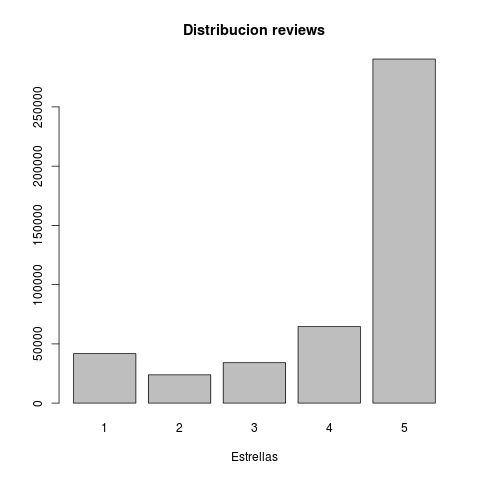
\includegraphics[width=1\linewidth]{Figures/dist_reviews.png}
\decoRule
\caption[Distribuci\'on de reviews]{Distribuci\'on de reviews con respecto a las clases.}
\label{fig:distribucion_reviews}
\end{figure}

La metodolog\'ia fue la siguiente:

\begin{itemize}
\setlength\itemsep{0em}
  \item Dividir los reviews de 5 estrellas en fracciones
  \item Por cada una de las fracciones
  \begin{itemize}
  \setlength\itemsep{0em}
    \item Mezclarla con los dem\'as reviews de 1-4 estrellas y entrenar la red con dicho set
  \end{itemize}
\end{itemize}

De esta forma se esperaba favorecer el aprendizaje sobre los reviews de valores menos frecuentes,
aunque los resultados mostraron que no hac\'ian una gran diferencia (en ning\'un caso hubo
siquiera una mejora).
